\documentclass[fleqn,b5paper,10pt]{article}

\usepackage{times,mathptmx,helvet}
\usepackage{graphicx} % use \usepackage[demo]{graphicx} to suppress figures
\usepackage{pdfsync}
\usepackage{amsmath}
\usepackage[justification=centering,labelsep=period,figurename=Figure,labelfont=bf]{caption}
\usepackage[sort&compress,square]{natbib}
\usepackage{url}
\usepackage{hyperref}
\usepackage[compact]{titlesec}
\usepackage{changepage} % to adjust right margin for abstract
\usepackage{array}
\usepackage{enumitem}
\usepackage{xcolor}
\usepackage{lipsum}
\usepackage{subcaption}

\setlength{\parindent}{0in}
\setlength{\parskip}{.5\baselineskip}
\setlength{\mathindent}{0cm}
\setlength{\labelsep}{10pt}

\titlespacing*{\section}
{0pt}{\baselineskip}{0pt}

\titleformat*{\section}
{\normalsize\bf}

\titlespacing*{\subsection}
{0pt}{\baselineskip}{0pt}

\titleformat*{\subsection}
{\normalsize\bf}

\titlespacing*{\subsubsection}
{0pt}{0pt}{0pt}

\titlespacing*{\paragraph}
{0pt}{\parskip}{5pt}

\hypersetup{colorlinks=true, urlcolor=blue, citecolor=black, linkcolor=black}
\urlstyle{same}

\captionsetup[table]{skip=5pt}
\captionsetup[figure]{skip=5pt}

%\usepackage[b5paper,showframe]{geometry} % use showframe option to help develop header/footer spacing
\usepackage[b5paper]{geometry}
\geometry{left=0.67in,right=0.67in,top=.67in,bottom=1.17in,headsep=.17in,foot=.17in}

% fancyhdr must come after geometry
\usepackage{fancyhdr}
\renewcommand{\headrulewidth}{0pt}
\renewcommand{\footrulewidth}{0pt}

\fancypagestyle{firststyle}
{
   \fancyhf{}
   \fancyfoot[L]{\footnotesize\sf\color{gray}\textit{Proc. of the Eleventh International Seminar on Fire and Explosion Hazards (ISFEH11), pp. xx-xx}\\
   Edited by J. Chao, V. Molkov, P. Sunderland, F. Tamanini and J. Torero\\
   Published by USTC Press\\
   ISBN: xxx-xxx-xx-xxxx-x :: doi: xx.xxxx/xxx-xxx-xx-xxxx-x\_0x-0x}
}

\fancyhf{}
\chead{\small\it\color{gray} Proc. of the Eleventh International Seminar on Fire and Explosion Hazards (ISFEH11)}
\cfoot{\color{gray}\thepage}
\pagestyle{fancy}


% single space between sentences
\frenchspacing

% ADD THE FOLLOWING COUPLE LINES INTO YOUR PREAMBLE
\let\OLDthebibliography\thebibliography
\renewcommand\thebibliography[1]{
  \OLDthebibliography{#1}
  \setlength{\parskip}{0pt}
  \setlength{\itemsep}{1pt}
}

%\renewcommand{\thefootnote}{\arabic{footnote}}
%\renewcommand{\labelitemi}{{\scriptsize $\bullet$}}
%\renewcommand{\labelitemii}{{\scriptsize $\bullet$}}

\newfont{\helvb}{phvb7t at 13pt} % helvetica narrow bold

\bibliographystyle{unsrtnat}
\setcitestyle{numbers,citesep={,\!}} % cite style is [1,2] instead of [1, 2] (remove space)

\begin{document}

\thispagestyle{firststyle}

\begin{center}
{\helvb Paper Title Using 13pt Arial Boldface Type and Initial Capitals}\\
\vskip\baselineskip
{\bf Student, A.\footnotemark[1], Student, B.\footnotemark[1]*, and Surname, C.\footnotemark[2]}\\
\vskip\baselineskip
{\it \footnotemark[1]Institution/Organization, Department, City, State/Province, Country.}\\
{\it \footnotemark[2]Institution/Organization, Department, City, State/Province, Country.}\\
{\it *Corresponding author email: \href{mailto:scientist@institution.com}{\underline{scientist@institution.com}}}\\
\end{center}

\subsection*{ABSTRACT}

\begin{adjustwidth}{0mm}{7mm}
{\small Insert your abstract here, retaining the formatting of this paragraph. It should include a concise (200-300 word) description of the results and findings of the research. It should not contain any reference or equation. Use 9 pt Times New Roman single spaced, making an indentation of 7 mm on the right margin. Include 3-4 keywords for indexing (in alphabetical order).

\paragraph{KEYWORDS:} Keyword1, keyword2, keyword3, keyword4.}
\end{adjustwidth}

\subsection*{NOMENCLATURE}

[This paragraph should be deleted in the final manuscript. If symbols are used extensively, a nomenclature listing, arranged alphabetically in a two-column format, must be included immediately following the Keywords. All {\it subscript} and {\it superscript} symbols appear separately. If units are provided, include them in parentheses. Use the international system (SI) of units. The example below can help you with the two-column formatting.]

\begin{tabular}{@{}ll}
\renewcommand{\tabcolsep}{15pt}
\begin{tabular}[t]{@{}ll}
$a$ & apparatus dimension (m) \\
$c_{\rm p}$ & heat capacity (J/kg/K) \\
$h$ & heat transfer coefficient (W/m$^2$/K)\\
$I$ & absorbed radiant heat flux (kW/m$^2$)\\
$L$ & glass thickness (m) \\
$l$ & decay length (m)\\
$q$ & heat flux (W/m$^2$)\\
$s$ & shaded length (m) \\
$T$ & temperature (K)\\
$T_0$ & ambient temperature (K)
\end{tabular}
&
\renewcommand{\tabcolsep}{15pt}
\begin{tabular}[t]{@{}ll}
$t$ & time (s)\\
$y$ & distance from edge (m)\\
$z$ & distance along edge (m)\\
\multicolumn{2}{@{}l}{\bf Greek}\\
$\epsilon$ & emissivity (-)\\
$\nu$      & thermal diffusivity (m$^2$/s)\\
\multicolumn{2}{@{}l}{\bf Subscripts}\\
L & ambient side of glass plane\\
0 & fire side of glass plane\\
\end{tabular}
\end{tabular}

\subsection*{MAIN HEADING}

Insert the body of your document here, retaining the formatting of this paragraph. All ISFEH paper submissions must follow this Word template. Use 10 pt Times New Roman fonts with justified margins. Do not change the paragraph attributes, paper size, margins, headers, or footers. Your paper {\bf must not exceed 10 pages}. Use a single space after each period.

Indicate references in the text using full-size consecutive numbers in brackets, i.e., \cite{McCaffrey:1981}. Include the full title in the references list (see below). The Reference style formats the indented paragraph and applies consecutive numbers.

Additional formatting instructions are below in ``Other Document Components.'' Refer to Appendix A for instructions on uploading your paper.

%%%%%%%%%%%%%%%%%%%%%%%%%%% ADD THIS AFTER FIRST PAGE %%%%%%%%%%%%%%%%%%%%%%%%%%%%%%%%%
\newgeometry{left=0.67in,right=0.67in,top=.77in,bottom=0.67in,headsep=.17in,foot=.17in}
\vspace*{-.67in} % may need to adjust this spacing
%%%%%%%%%%%%%%%%%%%%%%%%%%%%%%%%%%%%%%%%%%%%%%%%%%%%%%%%%%%%%%%%%%%%%%%%%%%%%%%%%%%%%%%

\subsection*{MAIN HEADING}

Continue body text here.

\subsubsection*{Supplementary Heading}

Continue body text here.

\subsection*{OTHER DOCUMENT COMPONENTS}

\subsubsection*{Abbreviations and acronyms}

Write out abbreviations or acronyms at their first mention in the text, followed by the abbreviation or acronym in parenthesis.

\subsubsection*{Equations}

For equations, \textbf{the size of all symbols MUST be set to 10 pt}. Number your equations consecutively in the text and refer to them as Eq.~(\ref{eqn_m}), etc. However, if ``Equation'' is the first word in a sentence, spell it out. Powers of e are often more conveniently denoted by exp. An Equation style has been provided, which includes a right aligned tab for the equation number and extra space after it. For example,
\begin{equation}
\label{eqn_m}
m(T_{\rm c}) = m_1(T_{\rm c}) + m_2(T_{\rm c}) = \frac{r+1}{2} \,\mbox{,}
\end{equation}
where $m$ is mass (kg), $r$ is radius (m), and $T$ is temperature (K).

Present simple formulae in line with normal text where possible and use the solidus ($/$) instead of a horizontal line for small fractional terms, e.g., $X/Y$.

\subsubsection*{Figures}

The ISFEH proceedings will be printed in grayscale (not color), so please ensure your figures are as comprehensible as possible without color printing. Each figure must have a number and a caption, as in the example below. The caption should be as concise as possible -- detailed information should be moved into the text. Figure captions should be centered below the figures. Number and refer to your figures consecutively, e.g., Fig.~\ref{fig_pyrolysis_model}. However, if ``Figure'' is the first word in the sentence, spell it out. Figures should be centered. In Word 2003 and 2007, figure objects should be inserted ``in line with text.''
\begin{figure}[h!]
\centering

\includegraphics[width=.5\linewidth]{isfeh_fig1.png}
\caption{Figure caption followed by period.}
\label{fig_pyrolysis_model}
\end{figure}

\begin{figure}[ht]
    \centering
    % First subfigure with fixed height
    \begin{subfigure}[b]{0.35\textwidth}
        \centering
        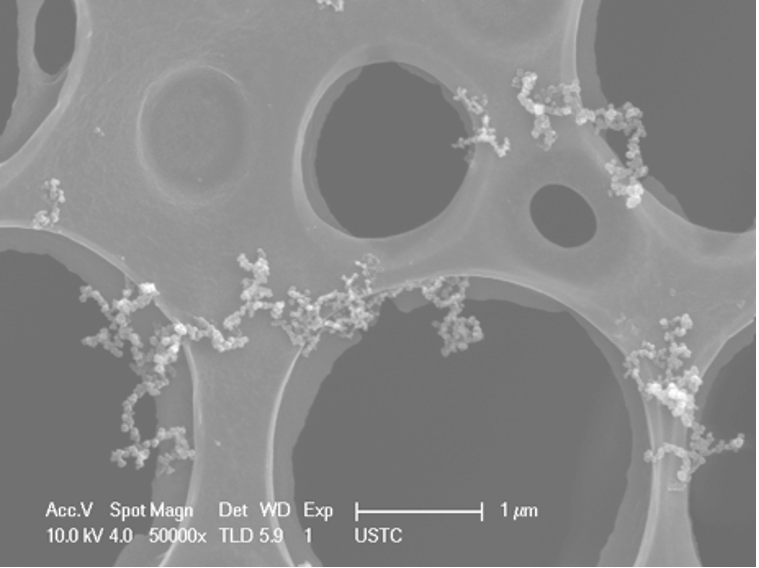
\includegraphics[height=4cm]{fig2a.png} % Replace with your image file and desired height
        \caption{}
        \label{fig:subfig1}
    \end{subfigure}
    \hspace{1cm} % Space between the two images
    % Second subfigure with the same fixed height
    \begin{subfigure}[b]{0.35\textwidth}
        \centering
        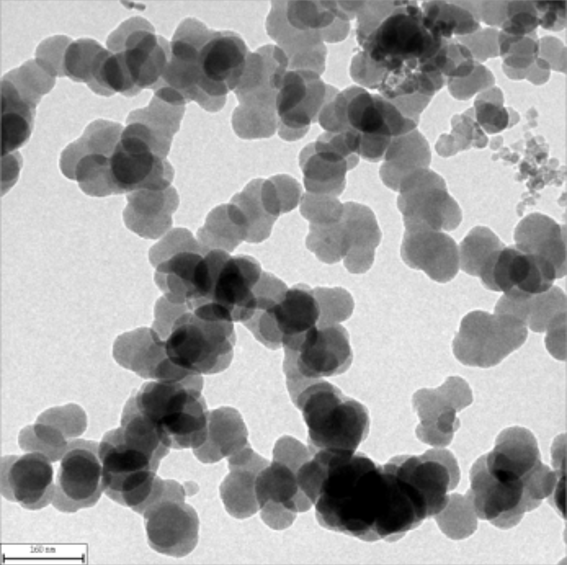
\includegraphics[height=4cm]{fig2b.png} % Replace with your image file and desired height
        \caption{}
        \label{fig:subfig2}
    \end{subfigure}
    % Main caption for the entire figure
    \caption{Characteristics of fire smoke particles. (a) SEM image; (b) TEM image.}
    \label{fig:smoke}
\end{figure}

\subsubsection*{Tables}

Each table must have a number and a title, as in the example below. The title should be as concise as possible -- detailed information should be moved into the text. Table titles should be centered above the tables. Number and refer to your tables consecutively, e.g., Table \ref{example_table}. Tables should be centered and should not include vertical rules.

\begin{table}[h]
\begin{center}
\caption{Table title followed by period.}
\small
\renewcommand{\arraystretch}{1.2}
\begin{tabular}{lcr}
\hline
Column 1  & Column 2  & Column 3$^{\mbox{\scriptsize b}}$ \\ \hline
\parbox[c]{.25\linewidth}{\vskip2pt Left align text in table rows for better legibility$^{\mbox{\scriptsize a}}$.}  & 31   & 499.6  \\
Sample text                                             & 30   &  88.8  \\
Sample text                                             & 29   & 516.5  \\
Sample text                                             & 29   &   6.4  \\ \hline
\multicolumn{3}{l}{$^{\mbox{\scriptsize a}}$Table footnotes are referenced by superscript letters.} \\[-.5ex]
\multicolumn{3}{l}{$^{\mbox{\scriptsize b}}$Decimal alignment of numbers in columns improves legibility.}
\end{tabular}
\label{example_table}
\end{center}
\end{table}

% Test longer document
%\lipsum
%\lipsum

\renewcommand{\refname}{\bf\normalsize REFERENCES}
% No brackets for the references
\makeatletter
\renewcommand\@biblabel[1]{#1.}
\makeatother

\nocite{McCaffrey:1981,Drysdale:1985,Heskestad:1995,Davis:2000}
\bibliography{ISFEH_refs}

\subsection*{APPENDIX A}
\label{app_a}

\subsubsection*{Uploading your paper to EasyChair}

\begin{enumerate}[align=left,leftmargin=*,labelsep=10pt]
\item Generate an Adobe Acrobat pdf version of your paper, embedding all fonts. You can choose any filename. You will also be required to upload an MS Word file or your \LaTeX source files.
\item Log in to the EasyChair site and select the appropriate ``Submission \#'' tab. In the top right  corner, select ``Update file''. You will then be prompted to upload your paper in both PDF and Word (or \LaTeX) formats.
\end{enumerate}


\end{document}
